% !TeX root = ../main.tex

\chapter{行人追踪算法}
  行人追踪算法blabla

  
\section{视觉行人追踪}
  计算机视觉中的行人追踪,主要包括密集跟踪方法,即基于行人检测和识别的追踪,以及稀疏跟踪方法,即基于目标动态的追踪。

  在密集跟踪方法中,我们实际上并没有“跟踪”物体,而是在视频不同的时间点的一系列帧上扫描和检测物体的位置。由于每次的目标检测都是独立地在当前帧上进行的,所以每次检测时,都需要处理图像中的所有像素,所以以这种方法进行目标跟踪,计算量会比较大。

  稀疏跟踪方法是根据物体的动态信息,对其可能的运动轨迹进行预测,并结合其上一帧所在位置和对当前帧的观察,得出其当前位置的算法。由于已知物体在上一帧时的位置,所以对当前帧识别时,只需要检测上一帧物体所在位置附近的像素,这样一来,相对于密集跟踪方法,就减少了大量的计算。此外,由于我们结合了对物体运动的预测和观察来进行估计,在一些情况下准确度也会较高,但在物体速度较快时,可能会失去对物体的追踪,当目标物暂时从视野中消失时,可能难以重新找回物体。

\subsection{基于检测的追踪}
  基于机器学习的方法是现阶段行人检测算法的主流,下面将介绍常用行人检测方法原理。

\subsubsection{人工特征+分类器}
\paragraph{常用特征描述子}

  特征描述子是一种对图片的表示方法,它通过提取图片中的关键信息并丢弃多余信息来对图片信息进行简化。通常地,特征描述子将一个RGB三通道的图片转化成一个特征向量。
  
  为了做到精确地进行图像识别、目标检测,我们必须首先明确什么是关键的、有用的信息,什么是冗余信息。

  a. 颜色直方图

  颜色特征具有旋转不变性,且不受目标的大小和形状的变化影响,在颜色空间中分布大致相同,从而具有较高的鲁棒性。

  颜色直方图是描述颜色特征最常用的描述子,它是是对目标表面颜色分布的统计,描述了不同色彩在图像中所占的比例,但无法描述图像中颜色的局部分布及每种色彩所处的空间位置,即无法描述图像中的某一具体的对象或物体。颜色直方图具有稳定性好、抗部分遮挡、计算方法简单和计算量小的特点。

  颜色直方图可以基于不同的的颜色空间,其中,最常用的是RGB空间和HSV空间。以RGB空间为例,分别统计每个像素的R、G、B数值落在[0,255]上每个点的频度,绘制出直方图,该图片的颜色特征即为三个长为256的向量,分别表示其的红色、绿色、蓝色的统计分布。以一张人物照片\ref{fig:ewan}为例,图\ref{fig:rgbhistogram}为其RGB颜色直方图。

\begin{figure}[htb]
  \centering
  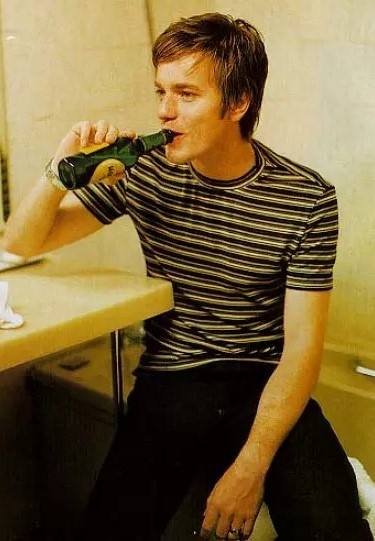
\includegraphics[width=0.3\textwidth]{ewan.jpg}
  \caption{原图}
  \label{fig:ewan}
\end{figure}

\begin{figure}[htb]
  \centering
  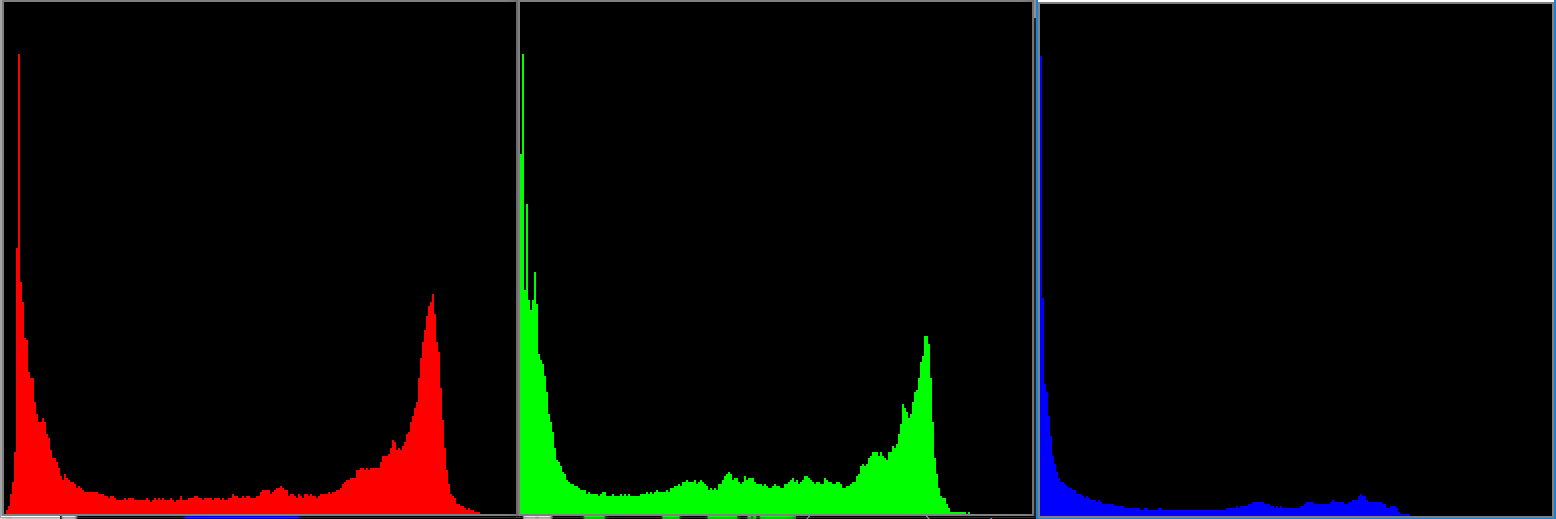
\includegraphics[width=0.6\textwidth]{rgb_histogram.png}
  \caption{左:B通道颜色直方图;中:G通道颜色直方图;右:R通道颜色直方图}
  \label{fig:rgbhistogram}
\end{figure}

  但RGB颜色空间的均匀性非常差,且两种颜色之间的直觉差异色差不能表示为改颜色空间中两点间的距离,RGB这三种颜色的分量的取值与所生成的颜色之间的联系并不直观。

  在计算机视觉中,我们常采用HSV颜色空间来表示颜色。HSV是一种将RGB色彩空间中的点在圆柱坐标系中的表示方法,相对于RGB,它能够更加直观地表示色彩的明暗、色调以及鲜艳程度,方便进行颜色之间的对比。此外,由于HSV单独提取了颜色的明暗,也可以一定程度上抵抗光照明暗带来的影响。\citet{sural2002segmentation}的实验显示,使用HSV直方图进行行人识别的结果相比RGB直方图有了明显提高。

  HSV即色相(Hue)、饱和度(Saturation)、亮度(Value)。色相即表示物体的颜色,如红色、黄色等,在$0^{\circ}$到$360^{\circ}$的标准色轮上,按位置度量色相;饱和度是指颜色的强度或纯度,表示色相中灰色分量所占的比例,它使用从0\%(灰色)至100\%(完全饱和)的百分比来度量;亮度是颜色的相对明暗程度,通常使用从0\%(黑色)至100\%(白色)的百分比来衡量。

\begin{figure}[htb]
  \centering
  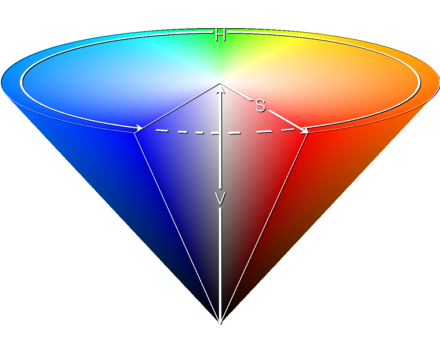
\includegraphics[width=0.3\textwidth]{hsv.png}
  \caption{HSV模型可以使用圆柱坐标系中的一个圆锥形子集表示}
  \label{fig:hsv}
\end{figure}

  由于大部分数字图像都是基于RGB空间进行表示的,我们需要首先把RGB空间坐标映射到HSV空间。给定$(r,g,b)$分别是一个颜色的红、绿、蓝坐标,它们的值是在0到1之间的实数,$max$为$r$,$g$和$b$之中的最大值,$min$为其中的最小值,则从$(r,g,b)$到$(h,s,v)$的转换公式如下:\cite{foley1982fundamentals}

$$h={\begin{cases}0^{\circ }&{\mbox{if }}max=min\\60^{\circ }\times {\frac  {g-b}{max-min}}+0^{\circ },&{\mbox{if }}max=r{\mbox{ and }}g\geq b\\60^{\circ }\times {\frac  {g-b}{max-min}}+360^{\circ },&{\mbox{if }}max=r{\mbox{ and }}g<b\\60^{\circ }\times {\frac  {b-r}{max-min}}+120^{\circ },&{\mbox{if }}max=g\\60^{\circ }\times {\frac  {r-g}{max-min}}+240^{\circ },&{\mbox{if }}max=b\end{cases}}$$

$$s={\begin{cases}0,&{\mbox{if }}max=0\\{\frac  {max-min}{max}}=1-{\frac  {min}{max}},&{\mbox{otherwise}}\end{cases}}$$

$$
v=max
$$

  HSV直方图的计算与RGB类似,只是将颜色空间有所差异,我们同样使用图片\ref{fig:ewan}计算其HSV直方图,见图\ref{fig:hsvhistogram}。

\begin{figure}[htb]
  \centering
  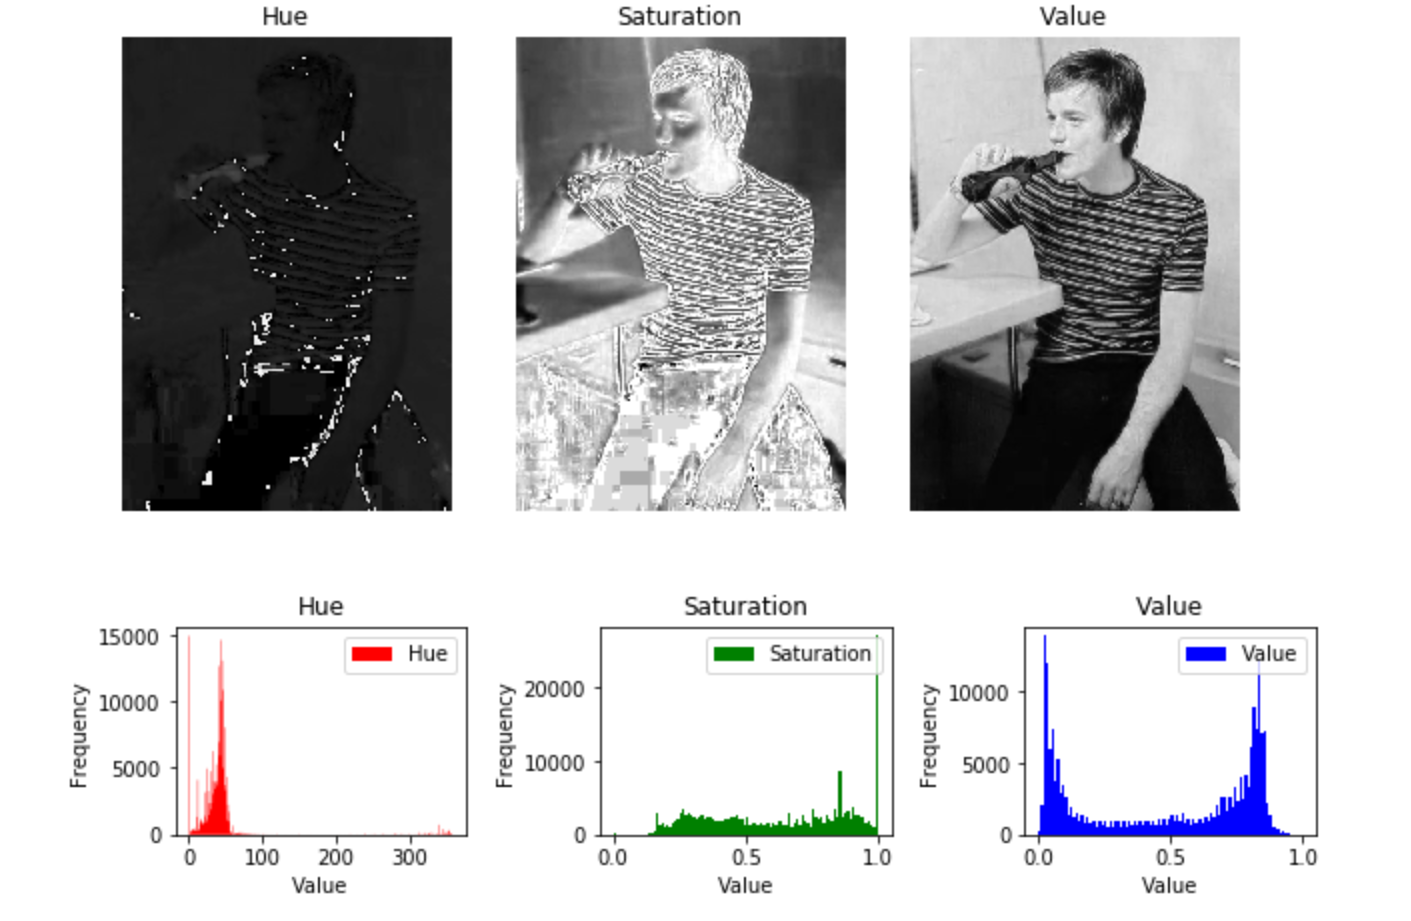
\includegraphics[width=1.0\textwidth]{hsv_histogram.png}
  \caption{左:H通道灰度图和颜色直方图;中:S通道灰度图和颜色直方图;右:V通道灰度图和颜色直方图}
  \label{fig:hsvhistogram}
\end{figure}

  b. 局部二值模式

  局部二值模式(Local Binary Pattern,LBP)是一种用来描述图像局部纹理特征的特征描述子,具有旋转不变性和对光照变化不敏感等优点,由\citet{ojala1994performance}在1994年首次提出。

  LBP的计算方法非常简单。每个像素都根据它相邻的八个像素按规定的顺序(如顺时针、逆时针)作比较,来确定其特征值。对于中心像素大于某个相邻像素的,该像素对应的二进制位设置为0,否则设置为1,比较了中心点相邻的八个像素后,就得到了一个8位的二进制数,这个数字即为中心像素的特征值,如图\ref{fig:lbp_procedure}所示,将每个点的LBP值使用灰度图表示,得到LBP图谱如\ref{fig:lbp}为例。

\begin{figure}[htb]
  \centering
  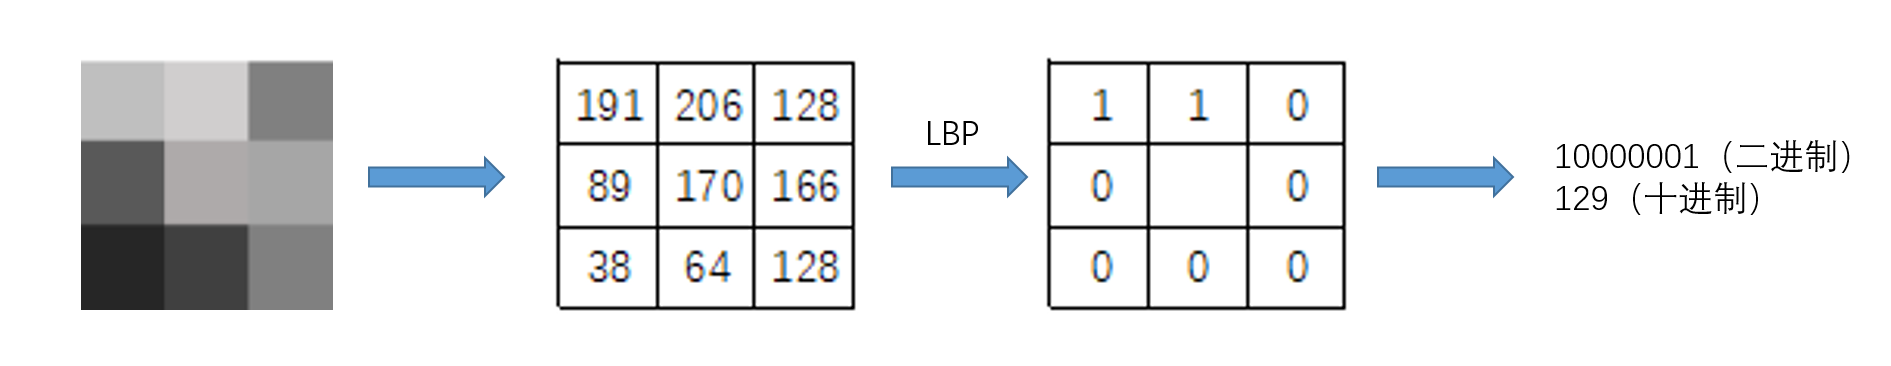
\includegraphics[width=0.9\textwidth]{LBP.png}
  \caption{计算3x3像素块中中心点的LBP值}
  \label{fig:lbp_procedure}
\end{figure}

\begin{figure}[htb]
  \centering
  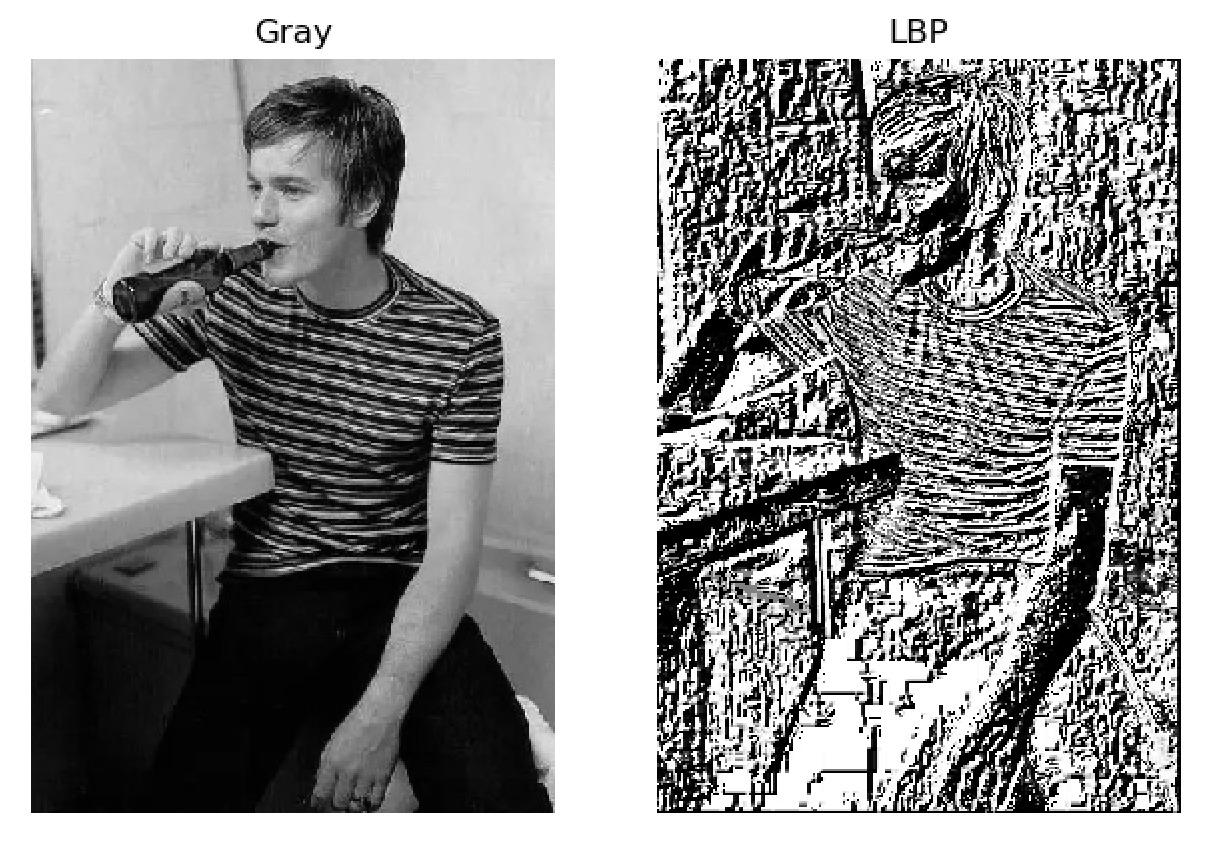
\includegraphics[width=0.6\textwidth]{ewan_lbp.png}
  \caption{左:灰度图;右:由灰度图计算得到的LBP图谱}
  \label{fig:lbp}
\end{figure}

  为了使得LBP描述子有旋转不变性,\citet{ojala2002multiresolution}提出了一个LBP的具有旋转不变性扩展方法,即不断旋转其邻域,得到一系列的LBP值,取其最小值作为该点的局部二值模式值。

  在计算一个图片的LBP描述子时,首先将图片分成固定大小的单元格(如$16\times16$像素),在计算出每个像素的LBP值后,统计每个单元格内的LBP值直方图,再串联所有单元格的直方图,即可得到该图片的LBP特征向量。



  c. 方向梯度直方图

  方向梯度直方图(Histogram of Oriented Gradient, HOG)是目前行人识别中最广泛使用的特征描述子之一。\citet{dalal2005histograms}在2005年提出HOG结合SVM(支持向量机,support vector machine)进行行人检测的方法,在此之后,该方法被广泛应用到了图像识别中,并尤其在行人检测中获得了巨大的成功,也出现了很多改进和变体。

  在HOG特征描述符中,它通过计算和统计图像局部区域的梯度方向直方图来构成特征。由于在物体的边缘和角落处图片的颜色会进行突变,故在这些区域,梯度的大小会很大,显然,边缘和角落比起平坦区域包含更多关于物体形状的信息。而通过对边缘和角度的描述,HOG正可以很好地描述局部目标的表面质地和形状信息。但同时,由于梯度的性质,HOG特征描述字对噪点比较敏感,且由于HOG主要描述了物体的轮廓,所以很难处理遮挡问题。

  为了计算方向梯度,我们可以简单地使用内核(Kernel)$[-1,0,1]$和$[-1,0,1]^{T}$对原图进行过滤,分别得到横向和纵向上的有向梯度。除了这种方法之外,还可以使用$[-1,1],[1,-8,0,8,-1]$和Sobel算子等作为内核,不过根据\citet{dalal2005histograms}的实验,使用最简单的$[-1,0,1]$进行计算的梯度,在以HOG为特征进行的图像识别中效果最佳。

  在每个像素处,方向梯度都具有大小和方向。对于彩色图像,我们分别计算RGB三个通道的梯度。对原图片上的每个像素点$(x,y)$,$f(x,y)$为其R、G、B值中的一个,该通道上的横向和纵向方向梯度为:
\begin{gather*}
g_x(x,y)=[-1,0,1]\ast f(x,y)=-f(x+1,y)+f(x-1,y),\\
g_y(x,y)=\begin{bmatrix}
-1 \\
0 \\
1
\end{bmatrix}
\ast f(x,y) = -f(x,y+1)+f(x,y-1)
\end{gather*}

  梯度大小和方向分别为:
\begin{gather*}
|g(x,y)|=\sqrt{g_x (x,y)^2 + g_y (x,y)^2} \\
\theta (x,y)=\tan^{-1}\left(\frac{g_y(x,y)}{g_x(x,y)}\right)
\end{gather*}
  
  使用以上公式在RGB颜色空间上计算图\ref{fig:ewan}的梯度值,如图\ref{fig:gradients}所示。这张梯度图像已经省略了图中很多不必要的信息,如颜色几乎一致的背景,且在同时突出了人物的轮廓。

\begin{figure}[htb]
  \centering
  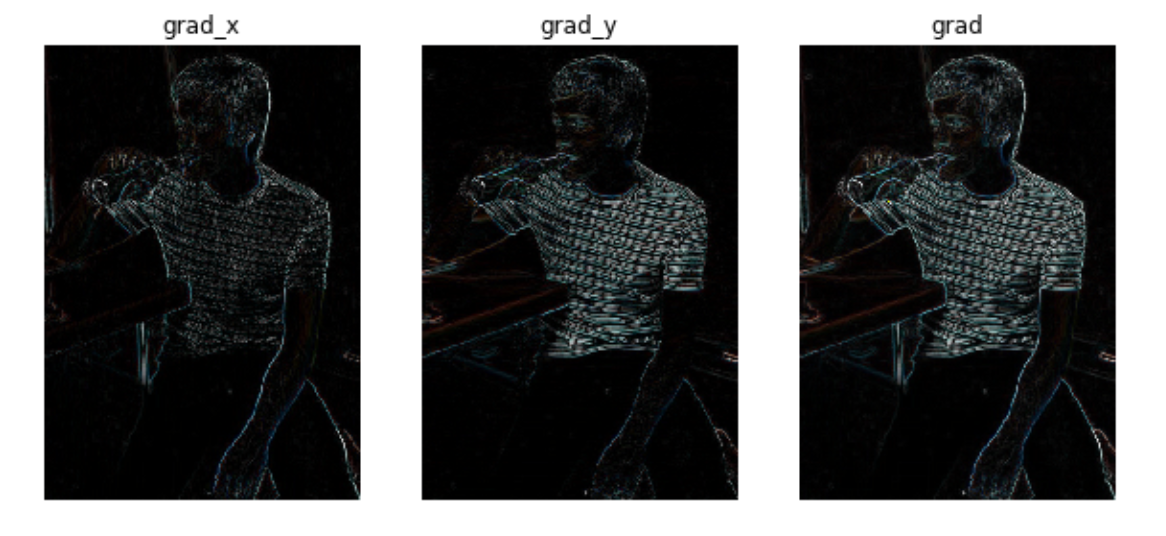
\includegraphics[width=0.9\textwidth]{gradients.png}
  \caption{左:横向梯度绝对值;中:纵向梯度绝对值;右:梯度大小}
  \label{fig:gradients}
\end{figure}

  图\ref{fig:gradients}中包括了RGB三个通道在每一个像素点上的梯度值,在计算HOG特征向量时,我们选取三个通道的梯度的最大值作为该点处的梯度大小,最大值对应的通道的梯度角度为该点处的梯度方向。

  方向梯度直方图统计的实际上是梯度的方向。梯度的方向在$[0^{\circ},360^{\circ})$上,但是我们实际在统计方向时,采用的却是$[0^{\circ},180^{\circ})$的统计范围,计算$\theta(x,y) \mod 180^{\circ}$来代替原有的角度值,即将相差$180^{\circ}$的两个角度视为同一个梯度方向。实验表明,这种统计方式得到的结果往往比采用$[0^{\circ},360^{\circ})$范围的原方向更好\cite{dalal2005histograms}。在统计梯度方向时时,我们还需要使用梯度的大小作为对应方向的权重。

  在计算直方图时,我们取9个组(bins),分别对应$0^{\circ},20^{\circ},40^{\circ},\dots,160^{\circ}$,若一个像素处的梯度正好为20的整数倍,将其梯度大小加到对应的bin中;否则,按照比例,将其加入相邻的两个bins中。以图\ref{fig:distribute}为例。这样一来,HOG特征描述子即为一个长为9的向量,每一个分量的大小对应直方图中相应bin的高度。

\begin{figure}[htb]
  \centering
  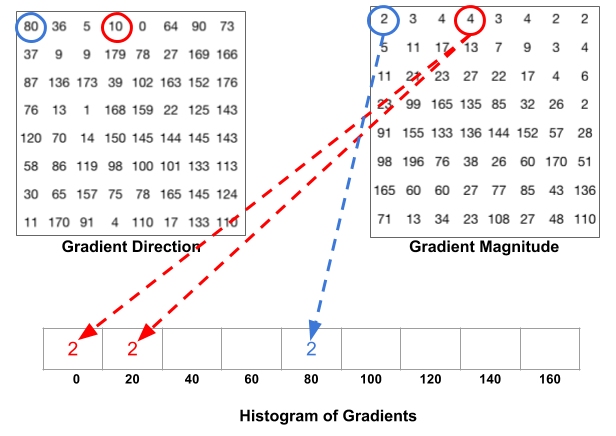
\includegraphics[width=0.7\textwidth]{calc_histogram.png}
  \caption{统计梯度方向直方图的方法示意}
  \label{fig:distribute}
\end{figure}

  值得注意的是,由于图像的梯度是由各像素点周围的颜色值大小计算得到的,所以也会受光照的影响,例如,将所有像素值除以2来使图像变暗,这时所有梯度大小就也会减半,直方图每个bin的高度也会减半。而在一张图片中,每个局部区域的光照可能会有所不同,为了降低这些影响,在进行方向梯度统计时,并不会直接统计一整个图片的方向梯度直方图,而是以$8\times8$像素的区域为一个单元格(cell)来分别进行统计,再在此基础上进行规范化(normalization)。这样会降低光照等噪音对特征描述子质量的影响,使HOG描述子更加稳定鲁棒。此过程如图\ref{fig:procedure}所示。

\begin{figure}[htb]
  \centering
  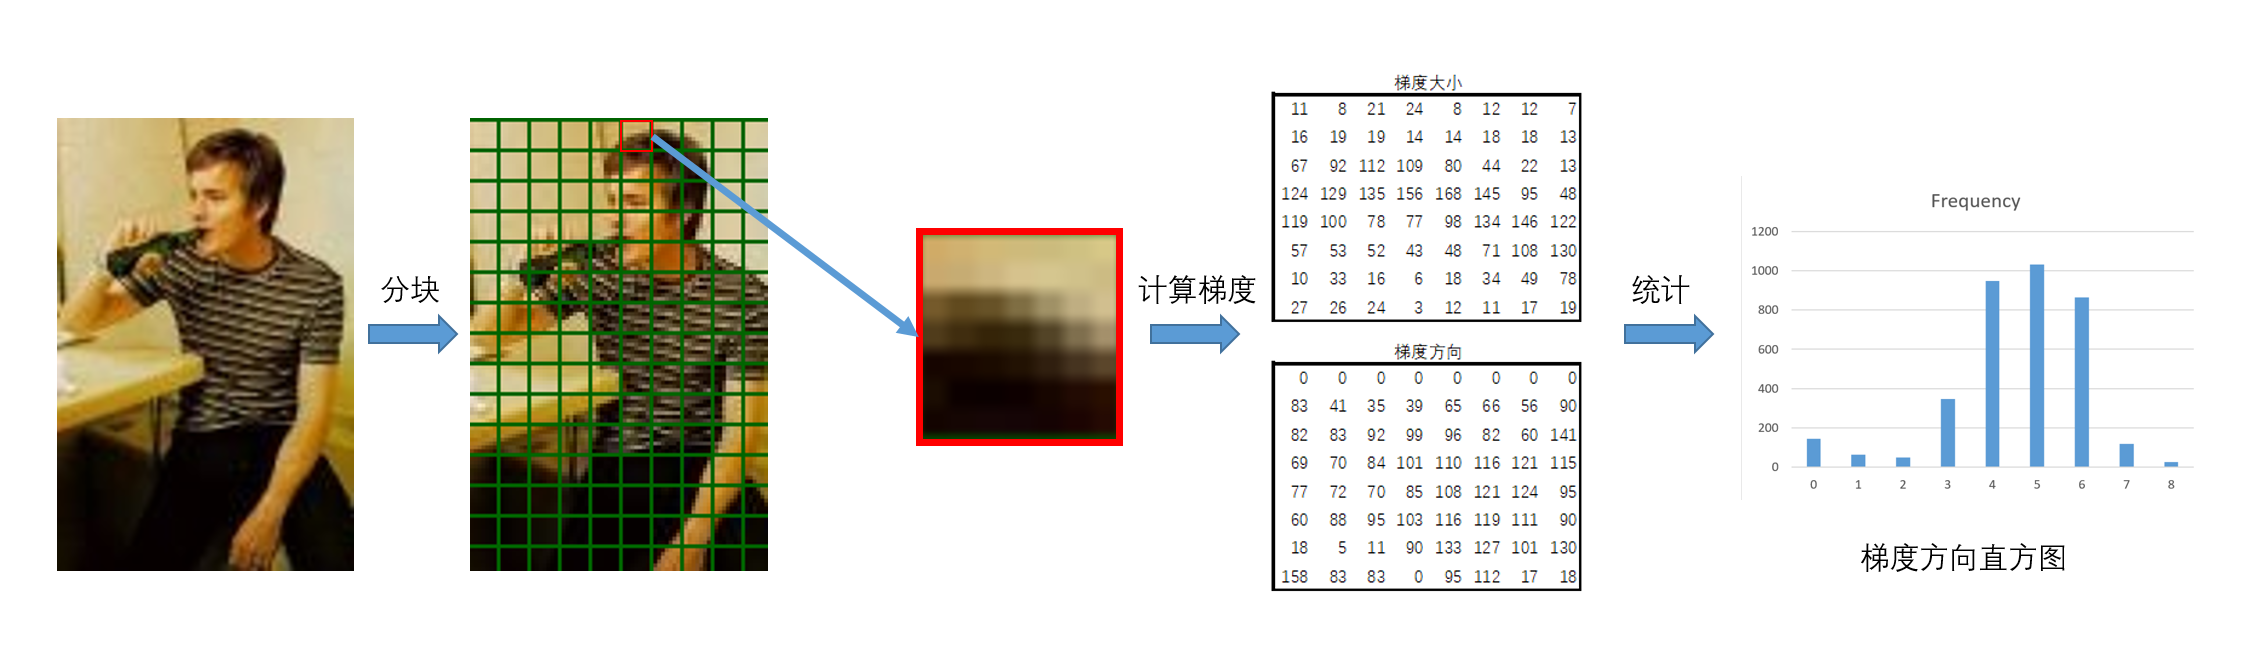
\includegraphics[width=1.1\textwidth]{procedure.png}
  \caption{统计单元格梯度直方图的过程示意图}
  \label{fig:procedure}
\end{figure}

  在进行规范化时,最常用的方法是在单元格的基础上取一个更大的块(block),每块的大小为$16\times16$像素,即包括4个单元格,将每一个块的4个HOG向量作为一个整体进行L2规范化。即$\vec{v}\leftarrow\vec{v}/\sqrt{\lVert v \rVert^2_2 + \epsilon^2}$,其中$\epsilon$为一个足够小的正常数。在规范化一个块之后,我们得到了一个长为36的向量,即这个块最终的HOG向量。再以8像素的步长(stride)移动这个块,对下一个块进行规范化,即两个相邻块之间有2个单元格的重叠。如此循环,直到整张图的每一个单元格都被计算,再将所有经过的块的向量合并在一起,作为整张图的HOG描述子。

  d. 尺度不变特征变换

  尺度不变特征变换(Scale-invariant feature transform,SIFT)是一种不受图片尺度和旋转影响,并在一定程度上不受光照和相机视角影响的特征描述子,它将图像数据转换为有关局部特征的尺度不变坐标。同时,通过在空间和频率域的准确定位,SIFT还可以减少遮挡和噪音带来的干扰。SIFT可以使用有效的算法从图片中提取出大量的独特特征,可以在所有的尺度和位置上密集地覆盖图像,例如,一个$500\times500$像素的图像可以最多生成2000个稳定的特征。SIFT方法中的关键点描述非常独特,可以使单个特征从大型特征数据库中能得到高概率的匹配。但在较为杂乱的图像中,背景中的很多特征可能不会从数据库中得到正确的匹配,故而在正确的匹配之外,生成错误的匹配,不过通过识别关于目标物及其在新图像中的位置,尺度和方向的关键点的子集,可以从完整匹配集中过滤出正确的匹配\cite{lowe2004distinctive}。

  为了最大限度地降低提取特征的成本,使用级联过滤(cascade filtering)方法来检测关键点,先使用高效的算法来检测出一些侯选位置,然后再进一步详细检查,将更加耗时的计算只运用到通过了初始测试的候选点位置。

  \citet{lowe2004distinctive}提出的SIFT生成图像特征的主要步骤如下:

  I. 尺度空间极值检测:通过高斯差分方程(difference-of-Gaussian function),在所有可能的尺度下搜索稳定的特征,来找出尺度和方向不变的潜在相关点。对于输入图像$I(x,y)$和可变尺度高斯核函数$G(x,y,\sigma)$,可以计算出图像的尺度空间$L(x,y,\sigma)$:
$$L(x,y,\sigma)=G(x,y,\sigma)\ast I(x,y)$$

  “$\ast$”为$x,y$上的卷积计算操作,$G(x,y,\sigma)=\frac{1}{2\pi\sigma^2}e^{-(x^2+y^2)/2\sigma^2}$,$\sigma$为尺度空间因子,反映了图像被模糊的程度,$\sigma$越大,对应的尺度也越大。

  为了有效地检测出尺度空间中稳定的关键点位置,使用高斯差分方程来与图像进行卷积,由一个常数因子$k$,得出$D(x,y,\sigma)$:
$$D(x,y,\sigma)=(G(x,y,k\sigma)-G(x,y,\sigma))\ast I(x,y)=L(x,y,k\sigma)-L(x,y,\sigma)$$

  为了检测中$D(x,y,\sigma)$函数的局部最大值和最小值,每个点都与它在同尺度上的8个邻点,以及相邻的两个尺度上的各9个邻点相比较(相邻尺度上$\sigma_{s+1}=k\dot\sigma_s$)。只有它的值比相比较的26个相邻点都要小或者都要大时,才选取该点作为候选点。

  II. 关键点精确定位:对每个候选点上,拟合一个精细的模型来确定其位置和尺度,并根据其稳定性来选择关键点。

  对尺度空间函数$D(x,y,\sigma)$进行最多二阶的泰勒展开:
$$D(\vec{x})=D+\frac{\partial D^T}{\partial \vec{x}}\vec{x}+\frac{1}{2}\vec{x}^T\frac{\partial^2D}{\partial\vec{x}^2}\vec{x}$$

  其中$D$和其微分在给定候选点处被计算,$\vec{x}=(x,y,\sigma)^T$是相对于该点的偏移向量。为了求$D$的局部极值的位置,对上式求导并设$D'$为0,则极值的位置的偏移量$\hat{\vec{x}}$和$D$的局部极值点分别为:
\begin{gather*}
\hat{\vec{x}}=-\frac{\partial^2 D^{-1}}{\partial \vec{x}^2}\frac{\partial D}{\partial \vec{x}}\\
D(\hat{\vec{x}})=D+\frac{1}{2} \frac{\partial D^T}{\partial \vec{x}} \hat{\vec{x}}
\end{gather*}

  为了保证极值点的稳定性,需要剔除低对比度的极值点。若$|D(\hat{\vec{x}})|$的值小于0.03(假定每个像素的值的大小在$[0,1]$之间),则将该极值点舍弃。

  III. 方向赋值:根据局部的图像梯度方向,将一个或多个方向赋值给每个关键点位置。后续在该图像上进行的所有操作都将根据为每个特征所指定的方向、尺度和位置进行变换(transform),从而为这些特征提供方向、尺度不变性。

  得到了每个关键点的尺度$\sigma$后,由特征点为中心,计算出同一尺度下周围区域每个点$(x,y)$的梯度大小$m(x,y)$和方向$\theta(x,y)$:
\begin{gather*}
m(x,y)=\sqrt{(L(x+1,y)-L(x-1,y))^2+(L(x,y+1)-L(x,y-1))^2}\\
\theta(x,y)=\tan^{-1}((L(x,y+1)-L(x,y-1))/(L(x+1,y)-L(x-1,y)))
\end{gather*}

  使用直方图统计关键点邻域内像素对应的梯度方向和大小。

  IV. 生成特征描述子:校正旋转门主方向以确保旋转不变性,生成关键点描述子并进行归一化处理,以去除光照的影响。

  SIFT准确率较高,对于尺度和旋转不敏感,但由于求SIFT特征向量计算量较大,耗时较长,所以在需要实时图像识别时并不常被使用。

\paragraph{算法示例}
  a. HOG+SVM

  b. HOG-LBP

  https://ieeexplore.ieee.org/abstract/document/5459207/


\subsubsection{深度学习}
  随着深度学习的发展,通过神经网络提取特征得到了广泛的应用。https://www.jianshu.com/p/d94e558ebe26

\subsection{基于动态的追踪}
\subsubsection{卡尔曼滤波}

  卡尔曼滤波是一种假定目标物体的运动服从线性高斯分布,以此对目标的运动状态进行预测,将预测结果与观察模型进行比较,根据误差更新预测模型,估计物体的当前位置的方法。
  
  卡尔曼滤波器是一组提供最小二乘法的有效递归解的数学方程,它可以对于系统的过去、当前、甚至未来状态的进行估计\cite{welch1995introduction}。

  卡尔曼滤波器对离散时间的控制过程的状态$x\in \real^n$进行估计,该过程由以下线性随机差分方程控制:
$$x_{k+1}=\mat{A}_k x_k + \mat{B} u_k + w_k$$

  同时,提供了对系统当前状态的测量$z\in \real^m$:
$$z_k=\mat{H}_k x_k + v_k$$

  其中,随机变量$w_k$和$v_k$分别表示系统和测量误差,假定它们是互相独立的,并服从正态分布:
\begin{gather*}
p(w)\sim N(0,Q),\\
p(v)\sim N(0,R).
\end{gather*}
  
  $n\times n$的矩阵$\mat{A}$将系统在时间$k$和$k+1$时的状态相关联起来,不存在驱动函数或系统噪音。$n\times l$的矩阵$\mat{B}$将控制输入$u\in \real^l$与系统状态$x$相关联。$m\times n$的矩阵$\mat{H}$将系统状态和对系统的测量$z_k$相关联。

  我们根据时间$k$前的过程,计算$\hat{x}^{-}_k \in \real^n$作为为时间$k$时的先验(a priori)状态估计,并根据对系统状态的测量$z_k$计算后验(a posteriori)状态估计$\hat{x}_k \in \real^n$。我们将先验和后验估计误差定义为:
$$e^{-}_k \equiv x_k -\hat{x}^{-}_k, e_k \equiv x_k - \hat{x}_k. $$

  则先验和后验估计误差协方差分别为:
\begin{gather*}
P^{-}_k = E[e^{-}_k {e^{-}_k}^T],\\
P_k=E[e_k {e_k}^T]
\end{gather*}

  使用先验估计$\hat{x}^{-}_k$和实际测量$z_k$来计算后验状态估计$\hat{x}_k$:
$$\hat{x}_k = \hat{x}^{-}_k + \mat{K} (z_k - \mat{H}_k \hat{x}^{-}_k)$$

  在上式中,$\mat{H}_k \hat{x}^{-}_k$是根据先验估计对测量值的预测,$(z_k - \mat{H}_k \hat{x}^{-}_k)$被称为测量残差(residual)。残差反映了先验估计及预测方法相对于实际测量的插值。$n\times m$的矩阵$\mat{K}$是最小化后验误差协方差的增益(gain)。将上式代入求$P_k$的公式中,取结果相对于$\mat{K}$的导数,并设为0,可以求得:
$$\mat{K}=\frac{P^{-}_k \mat{H}^T_k}{\mat{H}_k P^{-}_k \mat{H}^T_k + \mat{R}_k}$$

  由上式可以得出,$R_k$为了测量误差协方差,当它趋于0时,$\mat{K}$越大,特别地:
$$\lim_{R_k \to 0} \mat{K}_k=\mat{H}^{-1}_k$$

  另外,当先验估计误差协方差$P^{-}_k$趋于0时,$\mat{K}$越小,特别地:
$$\lim_{P^{-}_k \to 0} \mat{K}_k=0$$

  所以,当测量误差协方差$R_k$约接近0时,实际测量$z_k$更加被取信,而预测的测量值$\mat{H}_k \hat{x}^{-}_k$更不被相信,而当先验估计误差协方差$P^{-}_k$趋近于0时则相反。
  
  现在我们就有了根据先验估计和测量计算后验状态估计的方法。后验状态估计反映了状态分布的数学期望,根据$w,v$的分布,状态概率分布也应当满足正态分布,而后验估计误差协方差则反映了状态分布的误差。故:
$$p(x_k|z_k)\sim N(E[x_k],E[(x_k-\hat{x}_k)(x_k-\hat{x}_k)^T])=N(\hat{x}_k,P_k)$$

  卡尔曼滤波分为两组方程:时间更新方程和测量更新方程。时间更新方程根据当前状态和误差协方差估计,预测下一时间的先验估计;测量更新方程用于根据所获得的新的测量,再结合先验估计来获取一个已优化的后验估计,这个后验估计又被传回时间更新方程。如此循环,完成一个预测-矫正的过程,以自动化地对模型进行更新,对状态进行估计。

  时间更新方程包括:
\begin{gather*}
\hat{x}^{-}_{k+1}=A_k \hat{x}_k + B u_k \\
P^{-}_{k+1}=A_k P_k A^T_k + Q_k
\end{gather*}

  测量更新方程包括:
\begin{gather*}
K_k=P^{-}_k H^T_k(H_k P^{-}_k H^T_k + R_k)^{-1} \\
\hat{x}_k = \hat{x}^{-}_k + K (z_k - H_k \hat{x}^{-}_k) \\
P_k = (I-K_k H_k)P^{-}_k
\end{gather*}

  $Q_k$和$R_k$均为常数,分别与$w$和$v$相关,估计误差协方差$P_k$和增益矩阵$K_k$将会在计算中迅速收敛,并保持不变。

\subsubsection{粒子滤波}
  首先对跟踪目标进行建模,并定义一种相似度度量确定粒子与目标的匹配程度。在目标搜索的过程中,它会先按照一定的分布(比如均匀分布或高斯分布)在全局撒一些粒子,统计这些粒子与目标的相似度,确定目标可能的位置。在可能性较高的位置上,下一帧加入更多新的粒子,确保在更大概率上跟踪上目标。

  跟踪速度很快,而且能解决目标的部分遮挡问题。

  可以对非线性、非高斯系统的动态进行建模。

  粒子滤波器(particle filters)是一种基于概率密度的粒子表示的顺序蒙特卡洛方法(sequential Monte Carlo methods),它可以应用在任意状态-空间模型,是传统的卡尔曼滤波的一般化方法\cite{arulampalam2002tutorial}。

\subsubsection{点云法}

\subsubsection{MeanShift和CamShift}

\subsubsection{相关滤波}

\subsubsection{压缩追踪}

\subsubsection{深度学习}

\section{激光行人追踪}


